%%=============================================================================
%% Setup
%%=============================================================================

\chapter{Opstelling}
\label{ch:setup}

%% Bespreken testapplicatie en business applicatie voor het onderzoek
In dit hoofdstuk wordt er dieper ingegaan op de verschillende onderdelen van het Pridiktiv platform\footnote{platform of 'solution stack': Een set van componenten en software subsystemen die een geheel vormen waarmee de business doelstellingen worden bereikt}. Met behulp van component diagrammen\footnote{Een component diagram is een UML diagram die visueel voorstelt hoe componenten samenwerken om een software systeem te vormen} worden de architectuur en interactie visueel voorgesteld.
\section{Client}
\subsection{Client: Backoffice applicatie}
De backoffice is een Angular CLI applicatie en bestaat functioneel uit twee grote delen. Er is een zorgplanner en takenplanner voor de hoofdverplegers/hoofdverpleegsters waar zij het takenpakket voor een patient kunnen samenstellen. Voor het management is er een dashboard die inzicht biedt in de operationele werking van het woonzorgcentrum. De applicatie is afhankelijk van een internetconnectie om te kunnen functioneren. Omdat offline functionaliteit voor deze applicatie niet relevant is, komt het in het onderzoek niet verder aan bod.
\subsection{Client: Mobiele applicatie}
De mobiele applicatie is net als de backoffice een Angular CLI applicatie maar gebundeld als een Cordova applicatie. De applicatie wordt gebruikt door verplegers/verpleegsters en zorgkundigen in woonzorgcentra voor het registreren van verschillende handelingen.

\begin{figure}[h]
\caption{Flow van de mobiele applicatie}
\centering
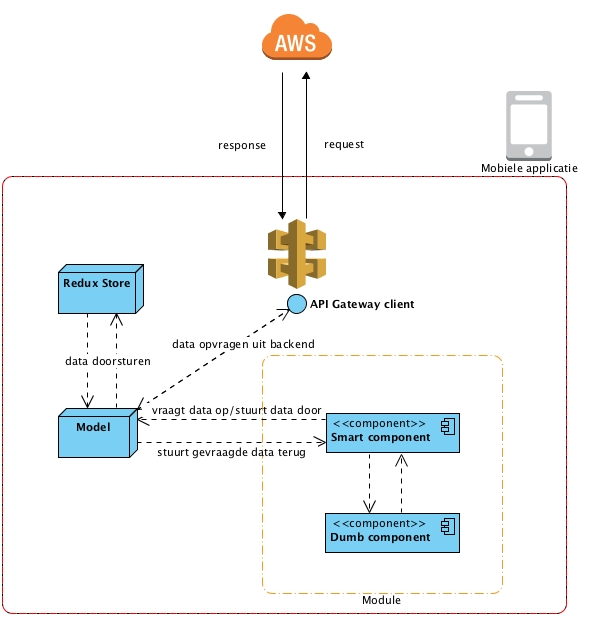
\includegraphics[width=0.9\textwidth]{mobile-overview}
\end{figure}

De applicatie maakt gebruik van verschillende design principes\autocite{brechtbilliet-scalable}\autocite{minko-gechev-scalable} die ervoor zorgen dat het een schaalbare Angular applicatie is. De applicatie bestaat uit verschillende Angular modules\footnote{Een Angular module is een verzameling van componenten en services. Modules organiseren een applicatie in coherente blokken van functionaliteit} die elke een feature voorstellen in de applicatie. 
\clearpage
Modules die data nodig hebben gebruiken een model\footnote{'model' verwijst in deze context naar een 'service' in Angular terminologie} voor het ophalen van de data uit de redux store. Indien de data niet in de store aanwezig is wordt die met behulp van de AWS API Gateway client opgevraagd aan de backend. De opgevraagde data wordt meteen in de store gestopt om het SSOT-principe te respecteren. Een smart component kan dan via zijn model data uit de redux store opvragen en stuurt die dan door naar een dumb component of meerdere dumb components. Wanneer er data wordt gewijzigd of gecree\"erd in een dumb component, stuurt het component de data terug naar zijn parent smart component. Via het model van de smart component wordt er in de store een nieuwe state gecree\"erd op basis van de nieuwe of aangepaste data.

Er wordt momenteel geen rekening gehouden met het cachen en precachen van data indien de applicatie plots offline is. Dit komt wel aan bod in het hoofdstuk ~\ref{ch:onderzoek} 'Onderzoek'
\section{Server}
De backend is opgebouwd volgens het 'serverless'\autocite{scalable-theorie} principe. Hierbij vormen AWS Lambda's de ruggengraat van de backend infrastructuur. Er wordt gebruik gemaakt van verschillende microservices die elk een beperkte maar specifieke verantwoordelijkheid hebben over een bepaalde functionaliteit. Voor de persistentie van de data wordt per data 'type'\footnote{Bijvoorbeeld pati\"enten en observaties zijn 2 verschillende datatypes} een DynamoDB tabel gebruikt. Met behulp van SNS kunnen Lambda's of andere AWS services op de hoogte worden gebracht wanneer er een neveneffect moet optreden bij het afhandelen van een request. De API Gateway is de toeganspoort tot de backend en is verantwoordelijk voor het delegeren van de binnenkomende requests. In de business case wordt er gebruik gemaakt van een proxy\footnote{Wanneer een lambda met proxy integration wordt gebruikt, hanteert de API Gateway een greedy 'catch-all' principe. Hierbij worden alle requests opgevangen en doorgestuurd naar de proxy lambda} lambda die de requests mapped naar de correcte lambda. Die voert dan de noodzakelijke stappen uit voor de request te verwerken.

\begin{figure}[h]
\label{fig:serverless}
\caption{Voorbeeld van een serverless architectuur opgezet met verschillende Amazon Web Services}
\centering
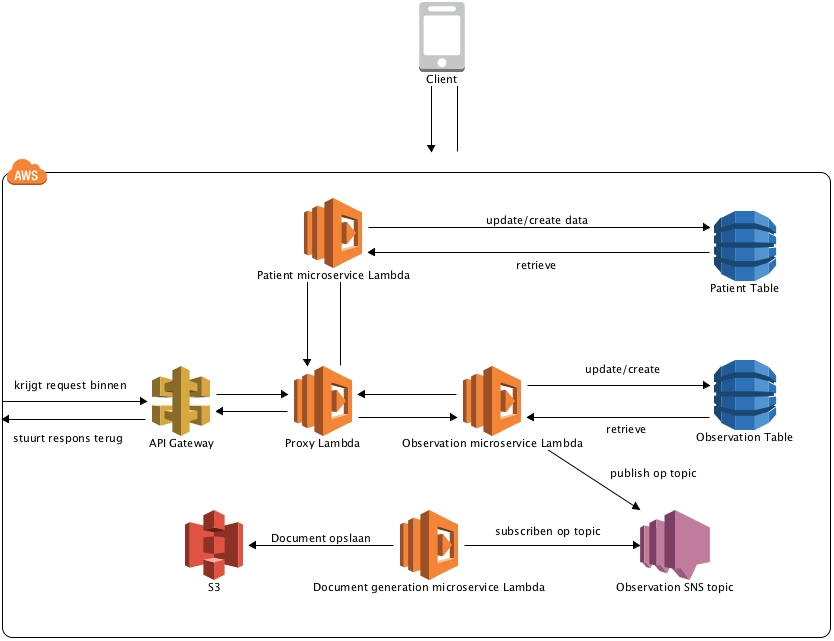
\includegraphics[width=0.9\textwidth]{serverless-example}
\end{figure}

Figuur~\ref{fig:serverless} is een voorbeeld van verschillende lambda's waarbij manipulaties worden uitgevoerd op patient -en observatiedata. De API Gateway stuurt een request naar de proxy lambda. Die triggert op zijn beurt de relevante lambda. Wanneer er een aanpassing gebeurt in de observatie data, plaatst de observatie microservice lambda een bericht op een SNS topic. Dit triggert dan de documentatie lambda die subscribed is op het SNS topic. Lambda en SNS werken dus perfect in tandem in het kader van een event-driven architectuur. 